\chapter{System Analysis and Design}


\begin{figure}
  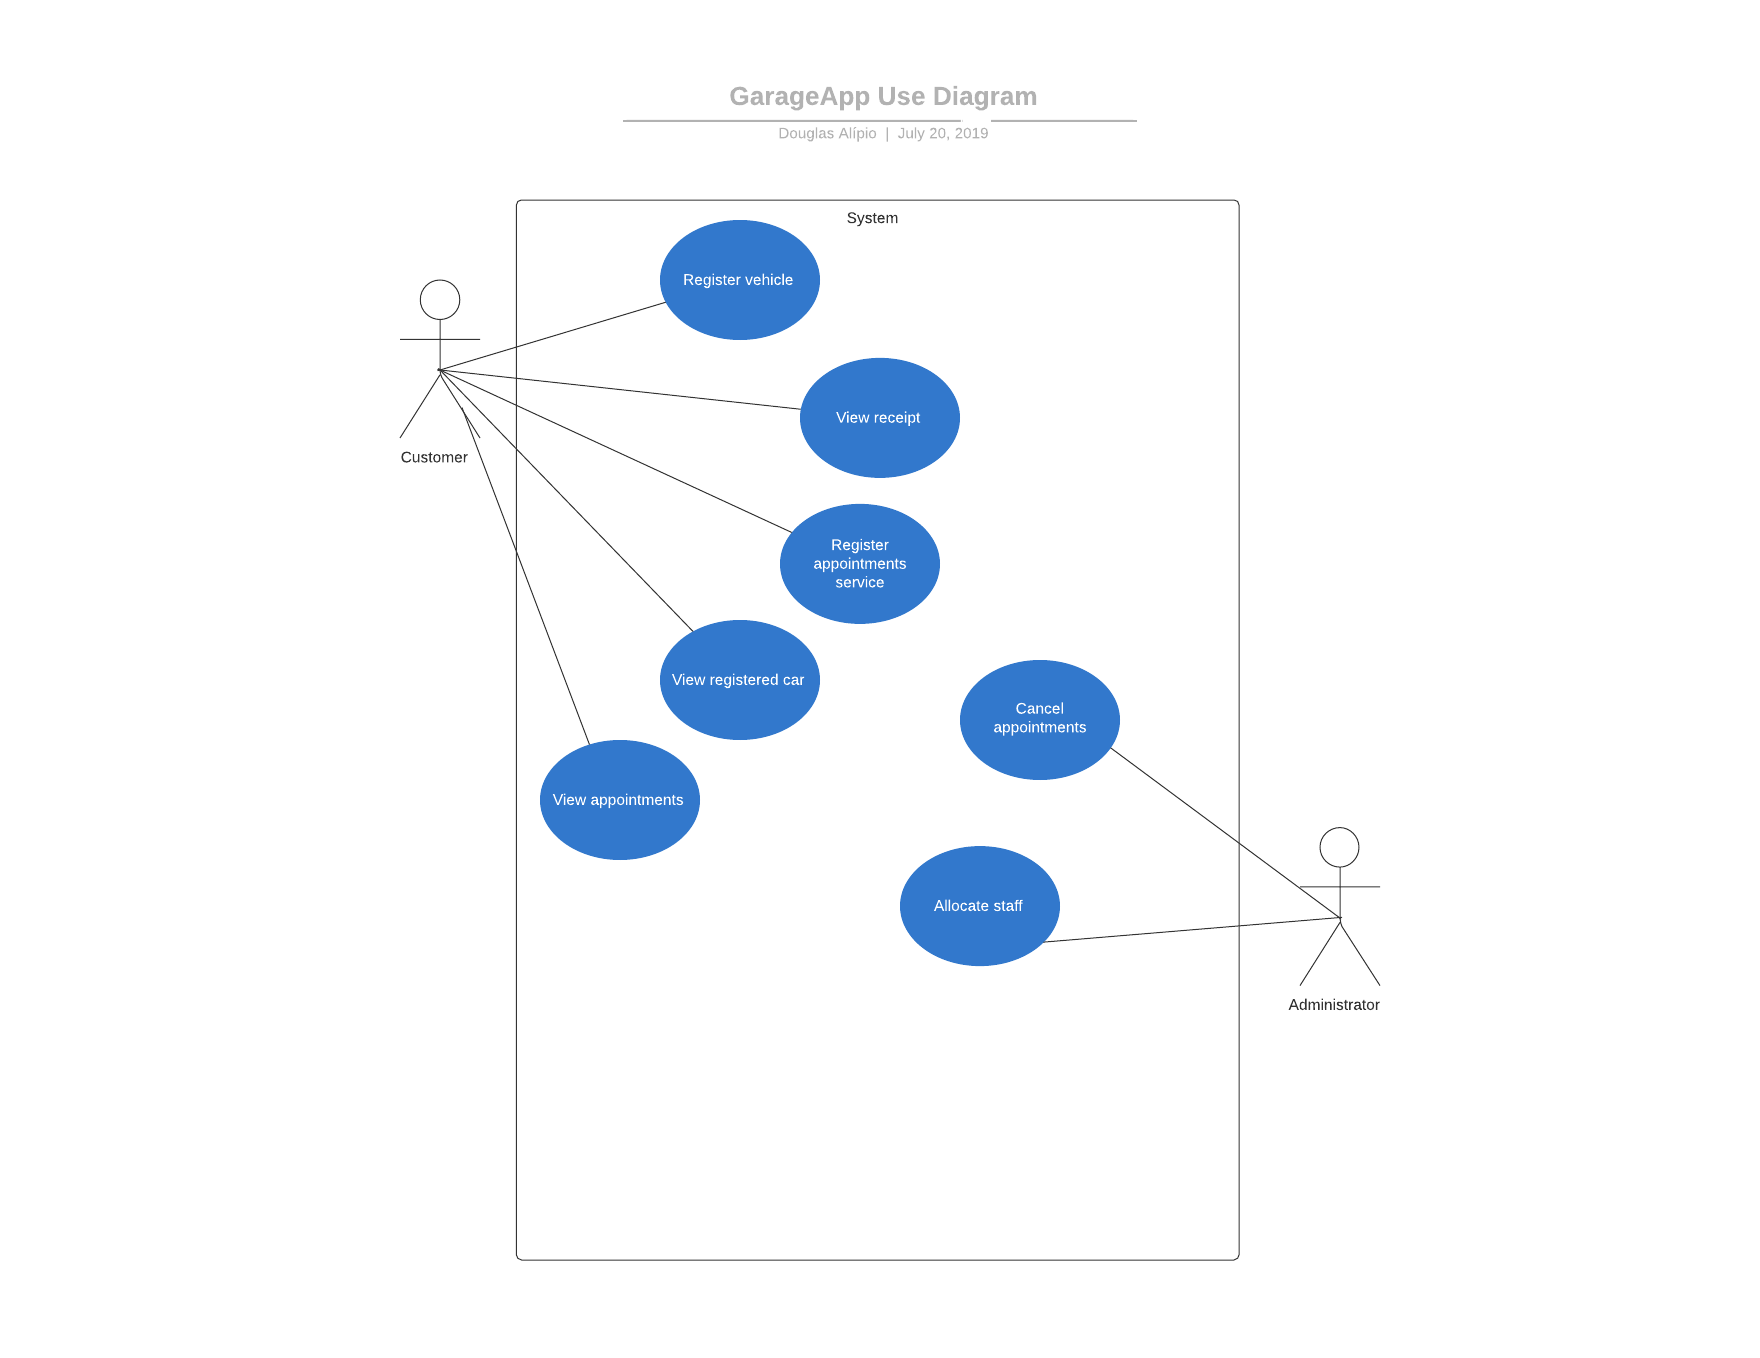
\includegraphics[width=\linewidth]{use_case_diagram.png}
  \caption{Use Case Diagram}
  \label{fig:diagram}
\end{figure}

The GarageApp is designed  to improve the user's experience to schedule appointment when they need to repair their vehicles. The application has a simple interaction which is log in into system, visualise the main screen and see the respective available dates and services. On the other hand, administrator of the system should be able to manage all appointments made by clients and allocate staff for each appointment.

\section{Functional Requirements for the Clients}

All requirements of the project is related to the client and administrator of the system. The most complex part comes from the client side. The model used to describe the requirements is based on Scrum methodology. Below all the most important requirements.

\begin{description}[font=$\bullet$~\normalfont\scshape\color{red!50!black}]

\item [Register vehicle] As user, I want to be able to register vehicle into system. The  basic information to make this action are registration number, make, model and mileage. Also, register max four vehicle. Vehicle types should be motorbikes, cars, small vans or small buses. If the vehicle are not this types, the system should reject the register showing a error message.

\item [View receipts]As user, I want to be able to see all receipts for service booked. The screen should show a list of receipts, when user click  one item a detail screen should show information about the specific receipt. The information are customer name, mobile number, vehicle and service price. If there is no available receipts, show only a blank list. At least, user can print any receipts.

\item [Book service] As user, I want to be able to book a service. The specific view should be compose by service type, date, vehicle and checkout button. The service  type must be annual service (€ 200), major service (€ 189), repair (€ 100), fault(€ 55). This feature is available only if user has internet connection, if not show a dialog error message.

\item [Log in] As user, I want to be able to log in and log out to the system. The screen should  show an email and password fields. If internet connection is available then user show the main screen, otherwise a dialog error message must be shown. After log out the system, it redirect user to log in screen.

\item [Log in] As user, I want to be able to log in to the system. The screen should  show an email and password fields. If internet connection is available then user show the main screen, otherwise a dialog error message must be shown.

\end{description}

\subsection{Functional Requirements for the administrator}

The system administrator is responsible to manage all appointments and allocate staff for a specific service. So the functional requirements are describe bellow.

\begin{description}[font=$\bullet$~\normalfont\scshape\color{red!50!black}]

\item [Cancel appointment] As admin, I want to be able to cancel any appointment on the system. The screen should show a list with all appointment and a confirmation/cancel button. If the administrator cancel it, the respective user must receiver a notification with the following message: "Unfortunately, your appointment [dd/mm/yyyy] was cancelled by the administrator. Would you like to make another one?".

\item [Allocate staff for a service]As admin, I want to be able to have a screen with all available staff. After click specific staff, another screen should show all appointments that the administrator can allocate the staff for the selected service.  After that action, the user must receiver a notification with the following message: "Congratulations! Your [service type] was confirm successfully".

\item [Book service] As user, I want to be able to book a service. The specific view should be compose by service type, date, vehicle and checkout button. The service  type must be annual service (€ 200), major service (€ 189), repair (€ 100), fault(€ 55). This feature is available only if user has internet connection, if not show a dialog error message.

\item [Log in] As user, I want to be able to log in and log out to the system. The screen should  show an email and password fields. If internet connection is available then user show the main screen, otherwise a dialog error message must be shown. After log out the system, it redirect user to log in screen.

\item [Log in] As user, I want to be able to log in to the system. The screen should  show an email and password fields. If internet connection is available then user show the main screen, otherwise a dialog error message must be shown.

\end{description}

\section{Another Section}

Phasellus nisi quam, volutpat non ullamcorper eget, congue fringilla leo. Cras et erat et nibh placerat commodo id ornare est. Nulla facilisi. Aenean pulvinar scelerisque eros eget interdum. Nunc pulvinar magna ut felis varius in hendrerit dolor accumsan. Nunc pellentesque magna quis magna bibendum non laoreet erat tincidunt. Nulla facilisi.

Duis eget massa sem, gravida interdum ipsum. Nulla nunc nisl, hendrerit sit amet commodo vel, varius id tellus. Lorem ipsum dolor sit amet, consectetur adipiscing elit. Nunc ac dolor est. Suspendisse ultrices tincidunt metus eget accumsan. Nullam facilisis, justo vitae convallis sollicitudin, eros augue malesuada metus, nec sagittis diam nibh ut sapien. Duis blandit lectus vitae lorem aliquam nec euismod nisi volutpat. Vestibulum ornare dictum tortor, at faucibus justo tempor non. Nulla facilisi. Cras non massa nunc, eget euismod purus. Nunc metus ipsum, euismod a consectetur vel, hendrerit nec nunc.